
\begin{appendices}
\setcounter{table}{0}
\setcounter{figure}{0}

\renewcommand{\thetable}{A\arabic{table}}
\renewcommand{\thefigure}{A\arabic{figure}}

\section{}\label{ap1}

\begin{figure}[H]
        \centering
        	\begin{minipage}{0.8\textwidth}	
                \caption{Rigiões Administrativas do estado de São Paulo}
                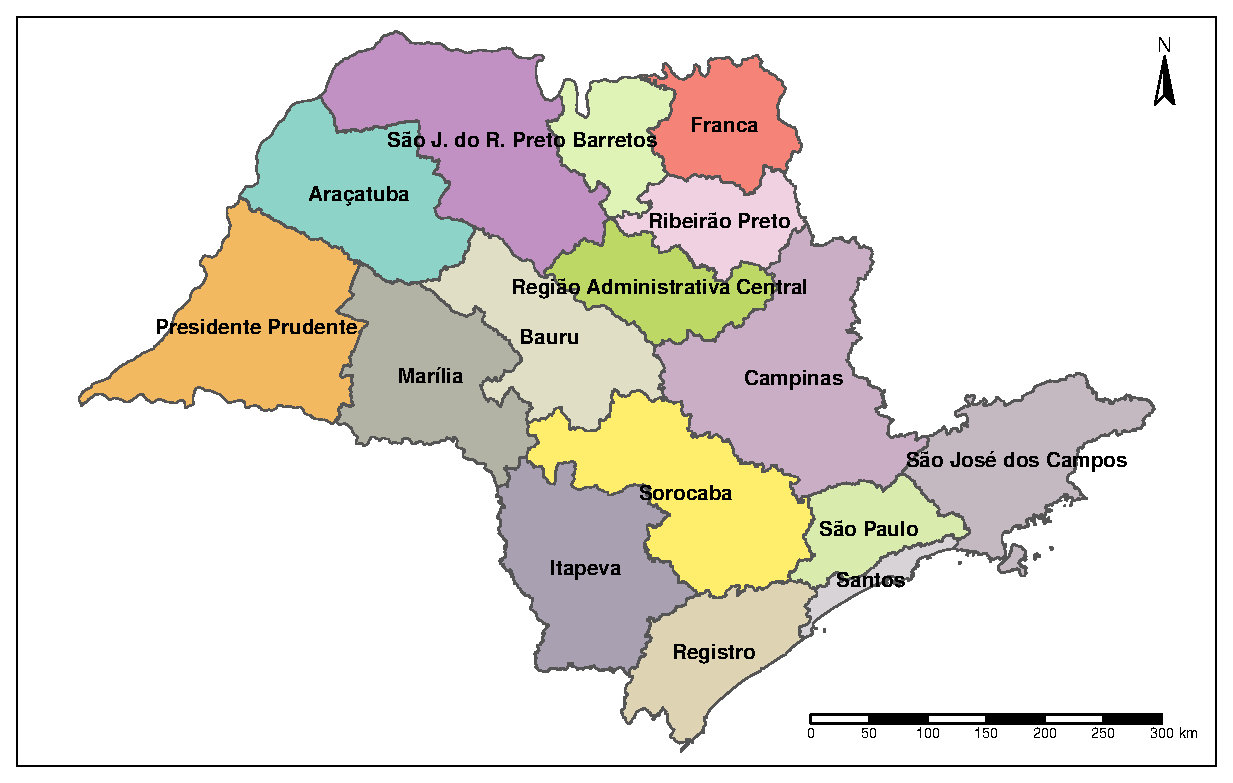
\includegraphics[scale=0.6]{figures/m2.eps}                 
            	\footnotesize \\
            		Fonte: Elaborado pelos autores.
    	\label{f:maps2}
	\end{minipage}
\end{figure}

\end{appendices}
